

\tikzset{every picture/.style={line width=0.3pt}} %set default line width to 0.75pt        

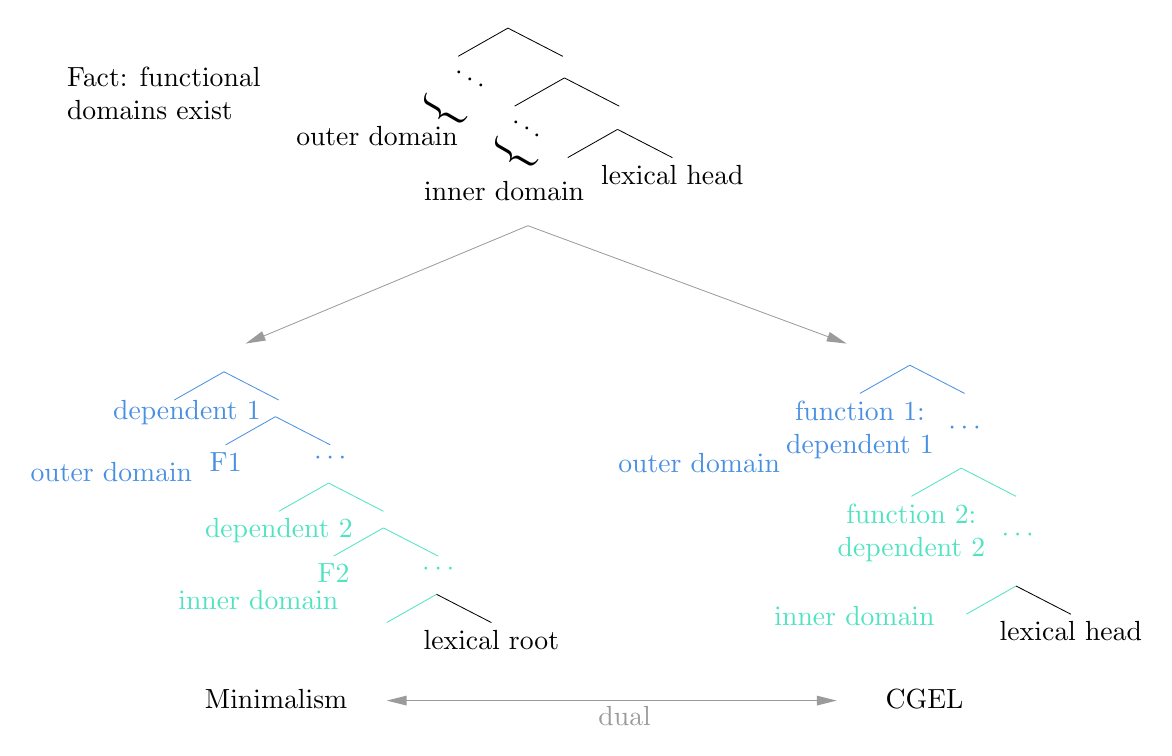
\begin{tikzpicture}[x=0.75pt,y=0.75pt,yscale=-0.8,xscale=0.8]
%uncomment if require: \path (0,523); %set diagram left start at 0, and has height of 523

%Straight Lines [id:da6705457534949089] 
\draw    (313,92.15) -- (343,75.15) ;
%Straight Lines [id:da28013820417559354] 
\draw    (376,92.15) -- (343,75.15) ;
%Straight Lines [id:da26185532929398736] 
\draw    (345,123.15) -- (375,106.15) ;
%Straight Lines [id:da1670225517468129] 
\draw    (408,123.15) -- (375,106.15) ;
%Straight Lines [id:da7951370858439135] 
\draw    (279,62.15) -- (309,45.15) ;
%Straight Lines [id:da5307564248915579] 
\draw    (342,62.15) -- (309,45.15) ;
%Straight Lines [id:da6264444449679678] 
\draw [color={rgb, 255:red, 155; green, 155; blue, 155 }  ,draw opacity=1 ]   (321,164.15) -- (152.85,234.38) ;
\draw [shift={(151,235.15)}, rotate = 337.33] [fill={rgb, 255:red, 155; green, 155; blue, 155 }  ,fill opacity=1 ][line width=0.08]  [draw opacity=0] (12,-3) -- (0,0) -- (12,3) -- cycle    ;
%Straight Lines [id:da99450357998767] 
\draw [color={rgb, 255:red, 80; green, 227; blue, 194 }  ,draw opacity=1 ]   (204,363.15) -- (234,346.15) ;
%Straight Lines [id:da7516847541397156] 
\draw [color={rgb, 255:red, 80; green, 227; blue, 194 }  ,draw opacity=1 ]   (267,363.15) -- (234,346.15) ;
%Straight Lines [id:da7086721116542554] 
\draw [color={rgb, 255:red, 80; green, 227; blue, 194 }  ,draw opacity=1 ]   (236,403.15) -- (266,386.15) ;
%Straight Lines [id:da23963037522787767] 
\draw    (299,403.15) -- (266,386.15) ;
%Straight Lines [id:da8629804052760564] 
\draw [color={rgb, 255:red, 74; green, 144; blue, 226 }  ,draw opacity=1 ]   (139,296.15) -- (146.67,291.8) -- (169,279.15) ;
%Straight Lines [id:da21212301774701436] 
\draw [color={rgb, 255:red, 74; green, 144; blue, 226 }  ,draw opacity=1 ]   (202,296.15) -- (169,279.15) ;
%Straight Lines [id:da45399705070135465] 
\draw [color={rgb, 255:red, 155; green, 155; blue, 155 }  ,draw opacity=1 ]   (321,164.15) -- (511.12,234.45) ;
\draw [shift={(513,235.15)}, rotate = 200.29] [fill={rgb, 255:red, 155; green, 155; blue, 155 }  ,fill opacity=1 ][line width=0.08]  [draw opacity=0] (12,-3) -- (0,0) -- (12,3) -- cycle    ;
%Straight Lines [id:da06579349148912339] 
\draw [color={rgb, 255:red, 80; green, 227; blue, 194 }  ,draw opacity=1 ]   (552,327.15) -- (582,310.15) ;
%Straight Lines [id:da7813158499201878] 
\draw [color={rgb, 255:red, 80; green, 227; blue, 194 }  ,draw opacity=1 ]   (615,327.15) -- (582,310.15) ;
%Straight Lines [id:da6554597016072419] 
\draw [color={rgb, 255:red, 80; green, 227; blue, 194 }  ,draw opacity=1 ]   (585,398.15) -- (615,381.15) ;
%Straight Lines [id:da38771820652223643] 
\draw    (648,398.15) -- (615,381.15) ;
%Straight Lines [id:da7029269298051468] 
\draw [color={rgb, 255:red, 74; green, 144; blue, 226 }  ,draw opacity=1 ]   (521,265.15) -- (528.67,260.8) -- (551,248.15) ;
%Straight Lines [id:da3078830979711833] 
\draw [color={rgb, 255:red, 74; green, 144; blue, 226 }  ,draw opacity=1 ]   (584,265.15) -- (551,248.15) ;
%Straight Lines [id:da5015548112989887] 
\draw [color={rgb, 255:red, 80; green, 227; blue, 194 }  ,draw opacity=1 ]   (171,336.15) -- (201,319.15) ;
%Straight Lines [id:da5954251542916287] 
\draw [color={rgb, 255:red, 80; green, 227; blue, 194 }  ,draw opacity=1 ]   (234,336.15) -- (201,319.15) ;
%Straight Lines [id:da4688878650352748] 
\draw [color={rgb, 255:red, 74; green, 144; blue, 226 }  ,draw opacity=1 ]   (108,269.15) -- (115.67,264.8) -- (138,252.15) ;
%Straight Lines [id:da2607503270176317] 
\draw [color={rgb, 255:red, 74; green, 144; blue, 226 }  ,draw opacity=1 ]   (171,269.15) -- (138,252.15) ;
%Straight Lines [id:da8702130416826466] 
\draw [color={rgb, 255:red, 155; green, 155; blue, 155 }  ,draw opacity=1 ]   (238,450.15) -- (505,450.15) ;
\draw [shift={(507,450.15)}, rotate = 180] [fill={rgb, 255:red, 155; green, 155; blue, 155 }  ,fill opacity=1 ][line width=0.08]  [draw opacity=0] (12,-3) -- (0,0) -- (12,3) -- cycle    ;
\draw [shift={(236,450.15)}, rotate = 0] [fill={rgb, 255:red, 155; green, 155; blue, 155 }  ,fill opacity=1 ][line width=0.08]  [draw opacity=0] (12,-3) -- (0,0) -- (12,3) -- cycle    ;

% Text Node
\draw (313.03,96.09) node [anchor=north west][inner sep=0.75pt]  [rotate=-30]  {$\cdots $};
% Text Node
\draw (408,126.15) node [anchor=north] [inner sep=0.75pt]   [align=left] {lexical head};
% Text Node
\draw (279.03,66.09) node [anchor=north west][inner sep=0.75pt]  [rotate=-30]  {$\cdots $};
% Text Node
\draw (42,67) node [anchor=north west][inner sep=0.75pt]   [align=left] {Fact: functional \\domains exist};
% Text Node
\draw (251.89,95.5) node [anchor=north west][inner sep=0.75pt]  [rotate=-300] [align=left] {{\LARGE \{}};
% Text Node
\draw (294.89,121.5) node [anchor=north west][inner sep=0.75pt]  [rotate=-300] [align=left] {{\LARGE \{}};
% Text Node
\draw (180,103) node [anchor=north west][inner sep=0.75pt]   [align=left] {outer domain};
% Text Node
\draw (257,136) node [anchor=north west][inner sep=0.75pt]   [align=left] {inner domain};
% Text Node
\draw (299,406.15) node [anchor=north] [inner sep=0.75pt]   [align=left] {lexical root};
% Text Node
\draw (20,305) node [anchor=north west][inner sep=0.75pt]  [color={rgb, 255:red, 74; green, 144; blue, 226 }  ,opacity=1 ] [align=left] {outer domain};
% Text Node
\draw (109,382) node [anchor=north west][inner sep=0.75pt]  [color={rgb, 255:red, 80; green, 227; blue, 194 }  ,opacity=1 ] [align=left] {inner domain};
% Text Node
\draw (139,299.15) node [anchor=north] [inner sep=0.75pt]  [color={rgb, 255:red, 74; green, 144; blue, 226 }  ,opacity=1 ] [align=left] {F1};
% Text Node
\draw (204,366.15) node [anchor=north] [inner sep=0.75pt]  [color={rgb, 255:red, 80; green, 227; blue, 194 }  ,opacity=1 ] [align=left] {F2};
% Text Node
\draw (125,442.15) node [anchor=north west][inner sep=0.75pt]   [align=left] {Minimalism};
% Text Node
\draw (648,401.15) node [anchor=north] [inner sep=0.75pt]   [align=left] {lexical head};
% Text Node
\draw (374,300) node [anchor=north west][inner sep=0.75pt]  [color={rgb, 255:red, 74; green, 144; blue, 226 }  ,opacity=1 ] [align=left] {outer domain};
% Text Node
\draw (468,392) node [anchor=north west][inner sep=0.75pt]  [color={rgb, 255:red, 80; green, 227; blue, 194 }  ,opacity=1 ] [align=left] {inner domain};
% Text Node
\draw (521,268.15) node [anchor=north] [inner sep=0.75pt]  [color={rgb, 255:red, 74; green, 144; blue, 226 }  ,opacity=1 ] [align=left] {\begin{minipage}[lt]{57.07pt}\setlength\topsep{0pt}
\begin{center}
function 1:\\dependent 1\\
\end{center}

\end{minipage}};
% Text Node
\draw (552,330.15) node [anchor=north] [inner sep=0.75pt]  [color={rgb, 255:red, 80; green, 227; blue, 194 }  ,opacity=1 ] [align=left] {\begin{minipage}[lt]{57.07pt}\setlength\topsep{0pt}
\begin{center}
function 2:\\dependent 2
\end{center}

\end{minipage}};
% Text Node
\draw (171,339.15) node [anchor=north] [inner sep=0.75pt]  [color={rgb, 255:red, 80; green, 227; blue, 194 }  ,opacity=1 ] [align=left] {dependent 2};
% Text Node
\draw (115.67,267.8) node [anchor=north] [inner sep=0.75pt]  [color={rgb, 255:red, 74; green, 144; blue, 226 }  ,opacity=1 ] [align=left] {dependent 1};
% Text Node
\draw (202,299.15) node [anchor=north] [inner sep=0.75pt]  [color={rgb, 255:red, 74; green, 144; blue, 226 }  ,opacity=1 ] [align=left] {$\displaystyle \cdots $};
% Text Node
\draw (267,366.15) node [anchor=north] [inner sep=0.75pt]  [color={rgb, 255:red, 80; green, 227; blue, 194 }  ,opacity=1 ] [align=left] {$\displaystyle \cdots $};
% Text Node
\draw (584,281.15) node [anchor=north] [inner sep=0.75pt]  [color={rgb, 255:red, 74; green, 144; blue, 226 }  ,opacity=1 ] [align=left] {$\displaystyle \cdots $};
% Text Node
\draw (616,345.15) node [anchor=north] [inner sep=0.75pt]  [color={rgb, 255:red, 80; green, 227; blue, 194 }  ,opacity=1 ] [align=left] {$\displaystyle \cdots $};
% Text Node
\draw (535,442) node [anchor=north west][inner sep=0.75pt]   [align=left] {CGEL};
% Text Node
\draw (362,452.15) node [anchor=north west][inner sep=0.75pt]  [color={rgb, 255:red, 155; green, 155; blue, 155 }  ,opacity=1 ] [align=left] {dual};


\end{tikzpicture}
